\documentclass[fleqn,11pt]{wlscirep}
\usepackage[utf8]{inputenc}
\usepackage[T1]{fontenc}
\usepackage{physics}
\usepackage{subfigure}
\usepackage{amsfonts}
\usepackage{amsmath}
\usepackage{amssymb}
\usepackage{mathtools}
\usepackage{bm}
\usepackage{siunitx}
\usepackage{mathptmx}
\usepackage{hyperref}
% Color package
\usepackage{xcolor}
\DeclareSymbolFont{epsilon}{OML}{ntxmi}{m}{it}
\DeclareMathSymbol{\epsilon}{\mathord}{epsilon}{"0F}
% \bibliographystyle{naturemag}
\usepackage[bitstream-charter,cal=cmcal]{mathdesign}

\newcommand{\Ai}{\operatorname{Ai}}
\newcommand{\Bi}{\operatorname{Bi}}

% Meta Data
\title{Non-equilibrium Transitions in Sub/Second Harmonic Generation: Quantum Theory}

\author[1,*]{Kosala Herath}

\affil[1]{Advanced Computing and Simulation Laboratory (A$\chi$L), Department of Electrical and Computer Systems Engineering, Monash University, Clayton, Victoria 3800, Australia}

\affil[*]{kosala.herath@monash.edu}

%\keywords{Keyword1, Keyword2, Keyword3}

\begin{abstract}

{
  This article provides a condensed summary and replication of numerical results from a prior theoretical investigation by Drummond \textit{et al.} \cite{drummond1981} on a non-linear optical system with a mode coupled to its second harmonic. Within this study, a quantum statistical analysis of coherently driven sub/second harmonic generation within an optical resonator is described. Quantum fluctuations are analyzed through a Fokker-Planck equation employing a generalized Glauber-Sudarshan P-representation. Specifically, the analysis focuses on the fluctuation behavior proximate to instability points as predicted by semiclassical theory. Remarkably, the spectrum of the sub-harmonic field exhibits critical narrowing in close proximity to the threshold, indicative of a second-order phase transition. Additionally, at higher driving field intensities, the sub-harmonic spectrum separate into two distinct peaks. Furthermore, the second harmonic light spectrum demonstrates a similar separation below the threshold for hard mode oscillations. Notably, under certain conditions, the photon statistics of the emitted light may reveal photon antibunching phenomena. This understanding and manipulation of anti-bunched light are crucial for advancing various applications in quantum technology, including secure communication, computing, metrology, and imaging.
}

\end{abstract}

\begin{document}

\flushbottom
\maketitle

\thispagestyle{empty}

\section*{Introduction}

The advent of the laser in 1960 \cite{maiman1960} marked a significant milestone, introducing a coherent, high-intensity light source capable of probing matter with unprecedented precision \cite{franken1963}. This breakthrough also initiated a new era in optics, where man-made light fields could apply sufficiently strong electric fields to modify fundamental electronic and optical properties of materials, paving the way for the emergence of non-linear optics \cite{bloembergen2000}.
The utilization of high-intensity lasers enables the exploration of optical non-linearities in materials, offering intriguing prospects for research and applications. Specifically, the investigation of harmonic generation, which involves both upconversion and downconversion frequencies, is pivotal within the realm of non-linear optics. The broad spectrum of applications for harmonic generation extends from contemporary photonics to the analysis and visualization of matter through spectroscopy and microscopy \cite{saleh2019,levenson2012,campagnola2002}.

Second harmonic generation, also known as frequency doubling, occurs when input photons interact with a nonlinear material and effectively combine to produce output photons with twice the frequency of the input photons. Conversely, subharmonic generation is a process where input photons divide to generate output photons with half the frequency of the input field \cite{franken1963,wang2023}. The theoretical analysis conducted by Drummond \textit{et al.} \cite{drummond1981} delved into sub-second harmonic generation within a coherently driven optical cavity, employing a comprehensive quantum mechanical framework. This investigation have described the possibility of non-classical statistics or photon antibunching in non-linear optical processes. While prior studies have addressed these quantum phenomena \cite{stoler1974,mostowski1978}, they  only focused on interacting modes not coupled to an external field, primarily considering transient situations. However, Drummond \textit{et al.} \cite{drummond1981} considered a non-linear crystal situated inside a driven optical cavity, thereby enabling the exploration of steady-state modes.

This review begins by outlining the system model and providing a quantum mechanical description, including the Hamiltonian for the non-linear optical process, which couples lower frequency electromagnetic field modes to higher frequency ones. Following standard procedure and employing the Markov approximation for the thermal baths \cite{louisell1973,walls2008}, the Hamiltonian is transformed into a master equation. Subsequently, by utilizing the Fokker-Plank equation in the complex P-representation \cite{drummond1980}, exact steady-state solutions are be derived. 

\section*{Theoretical Formalism}

In this investigation, we examine the dynamics of a non-linear crystal featuring a second-order susceptibility, situated within a Fabry-Perot interferometer configuration. Our focus lies on the interaction between two distinct light modes characterized by frequencies $\omega_1$ and $\omega_2$. We operate under the assumption that the frequency of the second light mode is approximately twice that of the first, $\omega_2 \approx 2\omega_1$. Both modes are subjected to external coherent phase-locked driving fields oscillating at frequencies $\omega_p$ and $2\omega_p$. This setup enables us to describe the mistuning with respect to the cavity resonance. Moreover, we account for mode damping resulting from cavity losses. Figure \ref{fig_system} presents a schematic representation of the resonant second-order non-linear optical system discussed herein. 
\begin{figure}[!t]
	\centering
	\subfigure{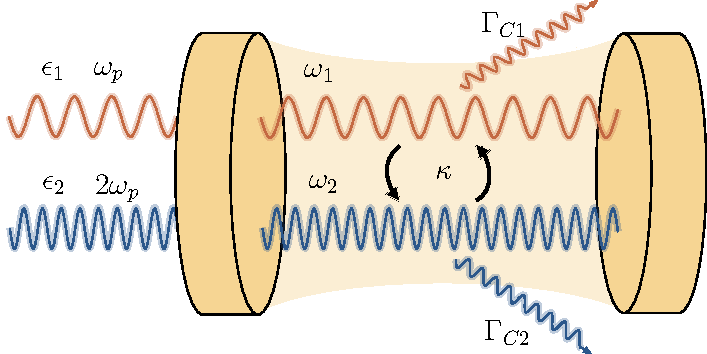
\includegraphics[width=0.5\textwidth]
	  {./figures/system.pdf}}
	\caption{The system comprises a cavity possesses two resonant light modes with frequencies $\omega_1$ and $\omega_2 \approx 2\omega_1$. External coherent driving fields with frequencies $\omega_p$ and $2\omega_p$ are applied to the system. The amplitude of each coherent driving field is denoted by $\epsilon_1$ and $\epsilon_2$. The operators $\hat{\Gamma}{c1}$ and $\hat{\Gamma}{c2}$ represent the heat bath annihilation operators characterizing the cavity losses associated with the two light modes. Furthermore, $\kappa$ is the coupling constant for the interaction between the two light modes.}
	\label{fig_system}
\end{figure}

The interacting Hamiltonian for the describing the system can be written as
\begin{equation}
	\hat{H} = \hat{H}_{\text{cav}} + \hat{H}_{\text{int}} + \hat{H}_{\text{pump}} + \hat{H}_{\text{bath}},
\end{equation}
where the Hamiltonian for the lights modes in the cavity is 
\begin{equation}
	\hat{H}_{\text{cav}} = \hbar\omega_1 \hat{a}_1^{\dagger}\hat{a}_1 +
	\hbar\omega_2 \hat{a}_2^{\dagger}\hat{a}_2,
\end{equation}
the interaction Hamiltonian is
\begin{equation}
	\hat{H}_{\text{int}} = i\hbar \frac{\kappa}{2}
	(\hat{a}_1^{\dagger\;2}\hat{a}_2 +
	\hat{a}_1^2\hat{a}_2^{\dagger}),
\end{equation}
the pumping Hamiltonian is
\begin{equation}
	\hat{H}_{\text{pump}} = 
	i\hbar(
		\epsilon_1\hat{a}_1^{\dagger}\exp(-i\omega_p t) - 
		\epsilon_1^{*}\hat{a}_1\exp(i\omega_p t)
	)
	+ i\hbar(
		\epsilon_2\hat{a}_2^{\dagger}\exp(-2i\omega_p t) - 
		\epsilon_2^{*}\hat{a}_2\exp(2i\omega_p t)
	),
\end{equation}
and the thermal bath Hamiltonian is
\begin{equation}
	\hat{H}_{\text{bath}} = 
	(\hat{a}_1 \hat{\Gamma}_{c1}^{\dagger} + \hat{a}_1^{\dagger}\hat{\Gamma}_{c1}) 
	+
	(\hat{a}_2 \hat{\Gamma}_{c2}^{\dagger} + \hat{a}_2^{\dagger}\hat{\Gamma}_{c2}).
\end{equation}
In this context, $\hat{a}_1$ and $\hat{a}_2$ represents the boson annihilation operators for the modes of frequency $\omega_1$ and $\omega_2$ respectively, $\kappa$ is the coupling contact for the light mode interaction. Moreover, the amplitude of the external driving field is denoted by $\epsilon_1$, and $\hat{\Gamma}{c1}$ and $\hat{\Gamma}{c2}$ represent the heat bath annihilation operators characterizing the cavity losses associated with the two light modes.

Following the standard procedures and tracing out the effects of the bath reservoirs \cite{louisell1973,walls2008}, the equation governing the density operator $\hat{\rho}$ of the two cavity modes can be found as 
\begin{equation}
	\begin{aligned}
		\pdv{\rho}{t} =&
			\frac{1}{i\hbar} [(\hat{H}_{\text{cav}} + \hat{H}_{\text{int}} + \hat{H}_{\text{pump}}),\hat{\rho}] +
			\gamma_1(2\hat{a}_1\hat{\rho}\hat{a}_1^{\dagger} - 
			\hat{a}_1^{\dagger}\hat{a}_1\hat{\rho}
			-\hat{\rho}\hat{a}_1^{\dagger}\hat{a}_1) +
			\gamma_2(2\hat{a}_2\hat{\rho}\hat{a}_2^{\dagger} - 
			\hat{a}_2^{\dagger}\hat{a}_2\hat{\rho}
			-\hat{\rho}\hat{a}_2^{\dagger}\hat{a}_2) \\
			&+ 2\gamma_1n^{\text{th}}_1
			(\hat{a}_1^{\dagger}\hat{\rho}\hat{a}_1 + 
			\hat{a}_1\hat{\rho}\hat{a}_1^{\dagger} -
			\hat{a}_1^{\dagger}\hat{a}_1\hat{\rho}-
			\hat{\rho}\hat{a}_1\hat{a}_1^{\dagger})
			+ 2\gamma_2n^{\text{th}}_2
			(\hat{a}_2^{\dagger}\hat{\rho}\hat{a}_2 + 
			\hat{a}_2\hat{\rho}\hat{a}_2^{\dagger} -
			\hat{a}_2^{\dagger}\hat{a}_2\hat{\rho}-
			\hat{\rho}\hat{a}_1\hat{a}_2^{\dagger}),
	\end{aligned}
\end{equation}
where $\gamma_1$ and $\gamma_2$ are the modes damping constants, and $n^{\text{th}}_1$ and $n^{\text{th}}_2$ are the thermal photon numbers of the baths. This master equation may be solved by various techniques \cite{louisell1973}. However, in this analysis we convert it to an associated $\mathcal{C}$-number equation. We map the master equation to $\mathcal{C}$-number Fokker-Planck
equation in the generalized P-representation \cite{walls2008} making the mapping: $(\hat{a}_1,\hat{a}_1^{\dagger},\hat{a}_2,\hat{a}_2^{\dagger}) \leftrightarrow ({\alpha}_1,{\alpha}_1^{+},{\alpha}_2,{\alpha}_2^{+})$. Then, we can identify that 
\begin{equation}
	\begin{aligned}
		\pdv{P(\boldsymbol{\alpha})}{t} =
		\Bigg\{&
			\pdv{\alpha_1}[(\gamma_1 + i\Delta_1)\alpha_1 - \epsilon_1 - \kappa\alpha_1^+\alpha_2]
			+
			\pdv{\alpha_1^+}[(\gamma_1 - i\Delta_1)\alpha_1^+ - \epsilon_1^* - \kappa\alpha_1\alpha_2^+]
			\\
			&\pdv{\alpha_2}[(\gamma_2 + i\Delta_2)\alpha_2 - \epsilon_2 + \frac{\kappa}{2}\alpha_1^2]
			+
			\pdv{\alpha_2^+}[(\gamma_2 - i\Delta_2)\alpha_2^+ - \epsilon_2^* + \frac{\kappa}{2}\alpha_1^{+\;2}]
			\\
			& \frac{1}{2}
			\Bigg[
				\pdv[2]{\alpha_1}(\kappa\alpha_2) 
				+ \frac{\partial^2}{\partial\alpha_1^{+\;2}}(\kappa\alpha_2^+)
				+ 2\gamma_1n^{\text{th}}_1\frac{\partial^2}{\partial\alpha_1\alpha_1^+}
				+ 2\gamma_2n^{\text{th}}_2\frac{\partial^2}{\partial\alpha_2\alpha_2^+}
			\Bigg]
		\Bigg\}P(\boldsymbol{\alpha}),
	\end{aligned}
\end{equation}
where $\boldsymbol{\alpha} = [{\alpha}_1,{\alpha}_1^{+},{\alpha}_2,{\alpha}_2^{+}]^{\intercal}$, $\Delta_1 = \omega_1 - \omega_p$ and $\Delta_2 = \omega_2 - 2\omega_p$. It is crucial to emphasize that in this generalized P-representation, $\alpha_{d}$ and $\alpha^+_{d}$ are not each other's complex conjugates where $d \in \{1,2\}$. Furthermore, it is important to mention that the following transformation to the rotating frames of the driving fields has been mode in the previous derivation:
\begin{equation}
	\alpha_1 \rightarrow \alpha_1\exp(-i\omega t), \quad \text{and} \quad
	\alpha_2 \rightarrow \alpha_2\exp(-2i\omega t).
\end{equation}
This enables us to establish equivalent stochastic differential equations employing the It$\hat{o}$ rules
\begin{equation}\label{eq_lan_1}
	\pdv{t}\mqty(\alpha_1 \\ \alpha_1^+) =
	\mqty(\epsilon_1 + \kappa\alpha_1^+\alpha_2 - (\gamma_1 + i\Delta_1)\alpha_1 \\
	\epsilon_1^* + \kappa\alpha_1\alpha_2^+ - (\gamma_1 - i\Delta_1)\alpha_1^+ ) +
	\mqty(\kappa\alpha_2 & 2\gamma_1n^{\text{th}}_1 \\
	 2\gamma_1n^{\text{th}}_1 & \kappa\alpha_2^+)^{1/2}
	\mqty(\eta_1(t) \\ \eta_1^+(t)),
\end{equation}
and 
\begin{equation}\label{eq_lan_2}
	\pdv{t}\mqty(\alpha_2 \\ \alpha_2^+) =
	\mqty(\epsilon_2 -\frac{\kappa}{2}\alpha_1^2 - (\gamma_2 + i\Delta_2)\alpha_2 \\
	\epsilon_2^* -\frac{\kappa}{2}\alpha_1^{+\;2} - (\gamma_2 - i\Delta_2)\alpha_2^+ ) +
	\mqty(0 & 2\gamma_2n^{\text{th}}_2 \\
	 2\gamma_2n^{\text{th}}_2 & 0)^{1/2}
	\mqty(\eta_2(t) \\ \eta_2^+(t)).
\end{equation}
Here, $\eta_d(t)$ and $\eta_d^+(t)$ are Gaussian random processes with the delta correlated relationship:
\begin{equation}
	\begin{aligned}
		&\expval{\eta_d(t)} = \expval{\eta_d^+(t)} = 0, \\
		&\expval{\eta_d(t)\eta_{d'}^+(t')} = \delta_{d,d'}\delta(t-t'),
	\end{aligned}
\end{equation}
where $\delta_{d,d'}$ is the Kronecker delta function and $\delta(t)$ is the Dirac delta function. 

\section*{Numerical Results}

To address the system of equations provided in Eq.~\eqref{eq_lan_1} and Eq.~\eqref{eq_lan_2}, we have two options: numerical integration or, where applicable, employing a linearized fluctuation analysis around the classical steady state solutions \cite{olsen2013}. Having previously solved these equations for classical steady state solutions in the previous work \cite{drummond1980n}, we opt for the second option in this current study. This will provide an opportunity to easily describe and predict both classical and quantum fluctuations in this system around the steady states.
A linearized fluctuation analysis can be executed by expressing the generalized P variables as the sum of a time-independent classical steady-state component and a time-dependent fluctuation variable, as described below:
\begin{equation}
	\alpha_d = \alpha_d^{\text{ss}} + \delta\alpha_d(t),
\end{equation}
where $\alpha_d^{\text{ss}}$ are the classical steady state solutions which can be found in Ref.~\cite{drummond1980n}. By substituting this back into the Eq.~\eqref{eq_lan_1} and Eq.~\eqref{eq_lan_2} we can identify new set of equations of motion for the fluctuation variables as follows
\begin{equation}
	\pdv{t}\delta\boldsymbol{\alpha} =
	-A \delta\boldsymbol{\alpha} + B \boldsymbol{\eta}(t),
\end{equation}
where $A$ is the steady state drift matrix which can be identify as
\begin{equation}
	A = \mqty(
		-\gamma_1 & \kappa\alpha_2^{\text{ss}} & \kappa \alpha_1^{\text{ss}\;*} & 0 \\
		\kappa \alpha_2^{\text{ss}\;*} & -\gamma_1 & 0 & \kappa\alpha_1^{\text{ss}} \\
		-\kappa\alpha_1^{\text{ss}} & 0 & -\gamma_2 & 0 \\
		0 & -\kappa\alpha_1^{\text{ss}\;*} & 0 & -\gamma_2
	),
\end{equation}
and $B$ is the matrix of the steady state coefficient for the fluctuations, as demonstrated by
\begin{equation}
	B = \mqty(
		\kappa\alpha_2^{\text{ss}} & 2\gamma_1n^{\text{th}}_1 & 0 & 0 \\
		2\gamma_1n^{\text{th}}_1 & \kappa\alpha_2^{\text{ss}} & 0 & 0 \\
		0 & 0 & 0 & 2\gamma_2n^{\text{th}}_2 \\
		0 & 0 & 2\gamma_2n^{\text{th}}_2 & 0
	)^{1/2}.
\end{equation}
In this context, $\delta\boldsymbol{\alpha} = (\delta\alpha_1,\delta\alpha_1^+,\delta\alpha_2,\delta\alpha_2^+)^{\intercal}$, and $\boldsymbol{\eta}(t) = (\eta_1(t),\eta_1^+(t),\eta_2(t),\eta_2^+(t))^{\intercal}$ \cite{olsen2013}. As long as the solutions are steady we can find the steady state spectrum of the cavity using the following expression \cite{drummond1980n,olsen2013} 
\begin{equation}\label{eq_spectrum}
	S(\omega) = \frac{1}{2\pi} (A + i\omega I)^{-1}D(A^{\intercal} - i\omega I)^{-1},
\end{equation}
where $D = BB^{\intercal}$, $I$ is the identity matrix, and $S(\omega)$ denotes the spectrum matrix, where its elements can be identified as the Fourier transform of the correction function
\begin{equation}
	S_{dd'}(\omega) = \frac{1}{2\pi} 
	\int_{-\infty}^{\infty} \exp(-i\omega \tau) \expval{\alpha_d(t)\alpha_{d'}(t+\tau)} \dd \tau.
\end{equation}
Since our primary focus is on quantum fluctuations, under this study we neglect thermal fluctuations in the system by setting $n^{\text{th}}_1 = n^{\text{th}}_2 = 0$. 

\subsection*{Sub Harmonic Generation}

First, using the Eq.\eqref{eq_spectrum} we can derive expression for the spectrum element $S_{12}(\omega) = \expval{\alpha_1(\omega)\alpha_1^+(\omega)}$ which is corresponds to the sub harmonic generation inside the cavity. substituting the $A$ and $B$ matrixes back into the Eq.~\eqref{eq_spectrum}, we can find a expression for the normalized spectrum $\tilde{S}_{12} = S_{12}/\gamma_2$ as follows
\begin{equation}
	\tilde{S}_{12}(\tilde{\omega}) = 
	\frac{
		\tilde{\alpha}_2^{\text{ss}\;2}(\tilde{\omega}^2 + 1)\left[\tilde{\alpha}_1^{\text{ss}\;2} + \tilde{\gamma}_1(\tilde{\omega}^2 + 1)\right]
	}{\pi \left[\mathcal{R}^2(\tilde{\omega}) + \mathcal{I}^2(\tilde{\omega})\right]},
\end{equation}
where we used the normalized variable: 
$\tilde{\alpha}_1^{\text{ss}} = \kappa{\alpha}_1^{\text{ss}}/\gamma_1$, 
$\tilde{\alpha}_2^{\text{ss}} = \kappa{\alpha}_2^{\text{ss}}/\gamma_2$, 
$\tilde{\gamma}_1 = \gamma_1/\gamma_2$, and 
$\tilde{\omega} = \omega/\gamma_2$. 
Furthermore, we introduced these functions for ease of notation
\begin{equation}
	\mathcal{R}(\tilde{\omega}) = 
	(\tilde{\alpha}_1^{\text{ss}\;2} + \tilde{\gamma}_1 - \tilde{\omega}^2 ) -
	\tilde{\omega}^2(\tilde{\gamma}_1 + 1)^2 -
	\tilde{\alpha}_1^{\text{ss}\;2}(1 - \tilde{\omega}^2),
\end{equation}
and 
\begin{equation}
	\mathcal{I}(\tilde{\omega}) = 
	2\tilde{\omega}
	\left[
	\tilde{\alpha}_2^{\text{ss}\;2} -
	(\tilde{\gamma}_1 +1)(\tilde{\alpha}_1^{\text{ss}\;2} + \tilde{\gamma}_1 - \tilde{\omega}^2 )
	\right].
\end{equation}
Since we consider the ub harmonic generation we can set $\epsilon_1 = 0$ and consider the spectrum under three different condition by changing the amplitude $\epsilon_2$ of the second light mode compared to the threshold $\epsilon_2^c = \gamma_1\gamma_2/\kappa$ for the second order phase transitions \cite{drummond1980n}. Figure \ref{fig_2} shows the spectrum of $\tilde{S}_{12}(\tilde{\omega})$ under the three conditions: $\epsilon_2$ is well below, just below and well above $\epsilon_2^c$. In this calculation we used the following classical steady state solutions as described in the previous literature \cite{drummond1980n,walls2008,mcneil1978}
\begin{equation} 
	\begin{aligned}
	&{\alpha}_1^{\text{ss}} = 0 \quad \text{and} \quad 
	{\alpha}_2^{\text{ss}} = \frac{\epsilon_2}{\gamma_2} \quad \text{when} \quad
	\epsilon_2 < \epsilon_2^c, \\
	&
	{\alpha}_1^{\text{ss}} = \pm \left[ \frac{2}{\kappa}(\epsilon_2 - \epsilon_2^c) \right]^{1/2} \quad \text{and} \quad 
	{\alpha}_2^{\text{ss}} = \frac{\gamma_1}{\kappa} \quad \text{when} \quad
	\epsilon_2 > \epsilon_2^c.
	\end{aligned}
\end{equation}
\begin{figure}[!t]
	\centering
	\subfigure{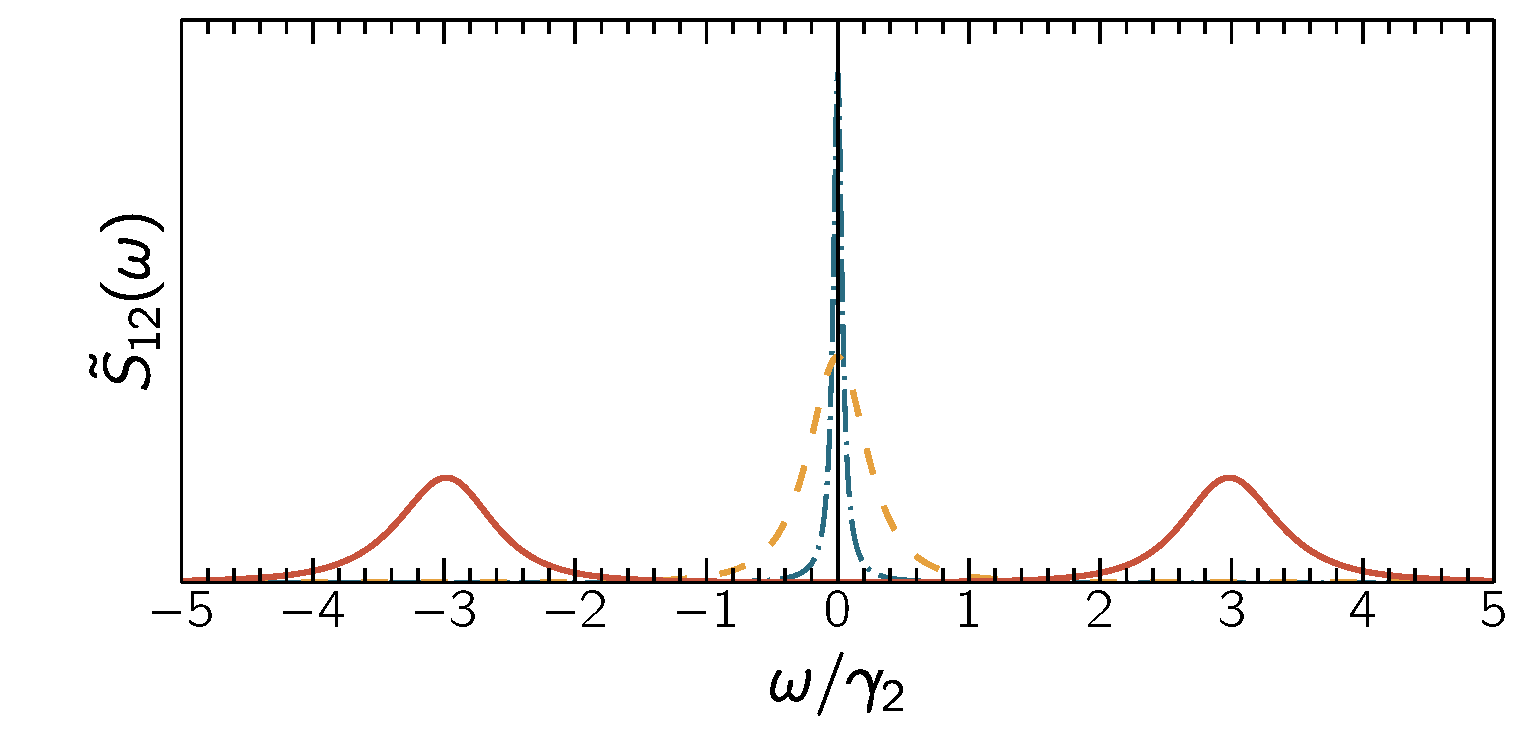
\includegraphics[width=0.6\textwidth]
	  {./figures/fig_2.pdf}}
	\subfigure{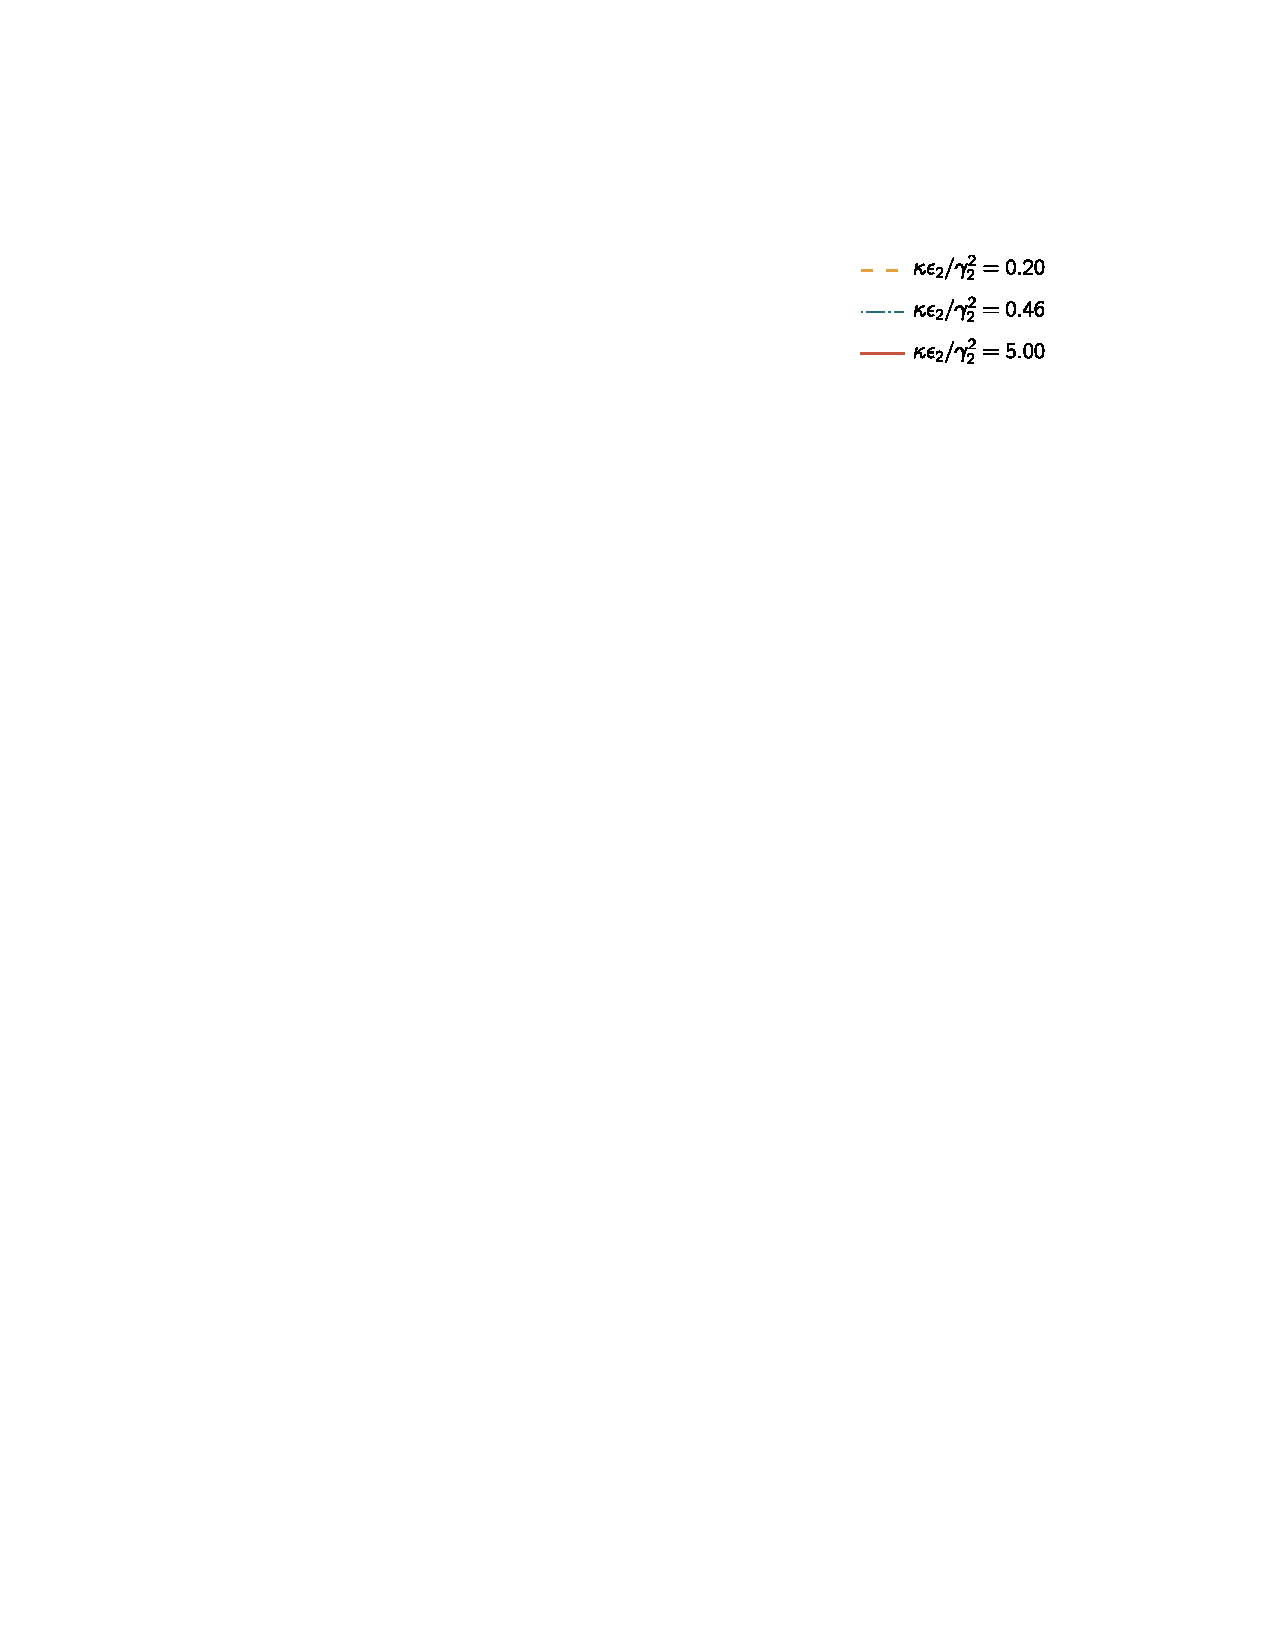
\includegraphics[width=0.18\textwidth]
	  {./figures/fig_2_legend.pdf}}
	\caption{Linearized spectrum $\tilde{S}_{12}(\tilde{\omega})$ for sub harmonic generation. Here, we assumed that $\gamma_1/\gamma_2 = 0.5$. Vertical scale ratios: 140:2:1.}
	\label{fig_2}
\end{figure}

\subsection*{Second Harmonic Generation}

In this subsection, we consider about the spectrum of the second harmonic generation $S_{34}(\omega) = \expval{\alpha_2(\omega)\alpha_2^+(\omega)}$.
Following the same steps as the previous subsection, we can derive an expression for the normalized spectrum for second harmonic generation  $\tilde{S}_{34} = S_{12}/\gamma_2$ as follows
\begin{equation}
	\tilde{S}_{34}(\tilde{\omega}) = 
	\frac{
		\tilde{\alpha}_2^{\text{ss}\;2}\tilde{\alpha}_1^{\text{ss}\;2}
		\left[\tilde{\alpha}_1^{\text{ss}\;2} + \tilde{\gamma}_1(\tilde{\omega}^2 + 1)\right]
	}{\pi \left[\mathcal{R}^2(\tilde{\omega}) + \mathcal{I}^2(\tilde{\omega})\right]}.
\end{equation}
Here, we set $\epsilon_2 =0$ to focus only on the second harmonic generation, and under different values of $\epsilon_1$ we can analyze the behavior of the spectrum. Figure \ref{fig_3} shows the behavior of spectrum for the second harmonic generation under three different values of $\epsilon_1$. It is imporatant to state that we only consider $\epsilon_1$ values that are lower then the threshold value $\epsilon_1^c$ which can be identify as \cite{mcneil1978} 
\begin{equation}
	\epsilon_1^c = \frac{\gamma_2 + 2\gamma_1}{\kappa}
	\left[ 2\gamma_2(\gamma_1 + \gamma_2)\right]^{1/2}.
\end{equation}
Following previous studies \cite{drummond1980n,mcneil1978}, we used following equation to find the classic stead state solution for ${\alpha}_2^{\text{ss}}$ variable for different levels of $\epsilon_1$ values 
\begin{equation}
	-\gamma_2(\kappa{\alpha}_2^{\text{ss}})^3 +
	4\gamma_1\gamma_2(\kappa{\alpha}_2^{\text{ss}})^2 -
	2\gamma_1^2\gamma_2(\kappa{\alpha}_2^{\text{ss}}) =
	|\kappa\epsilon_1|^2.
\end{equation}
\begin{figure}[!t]
	\centering
	\subfigure{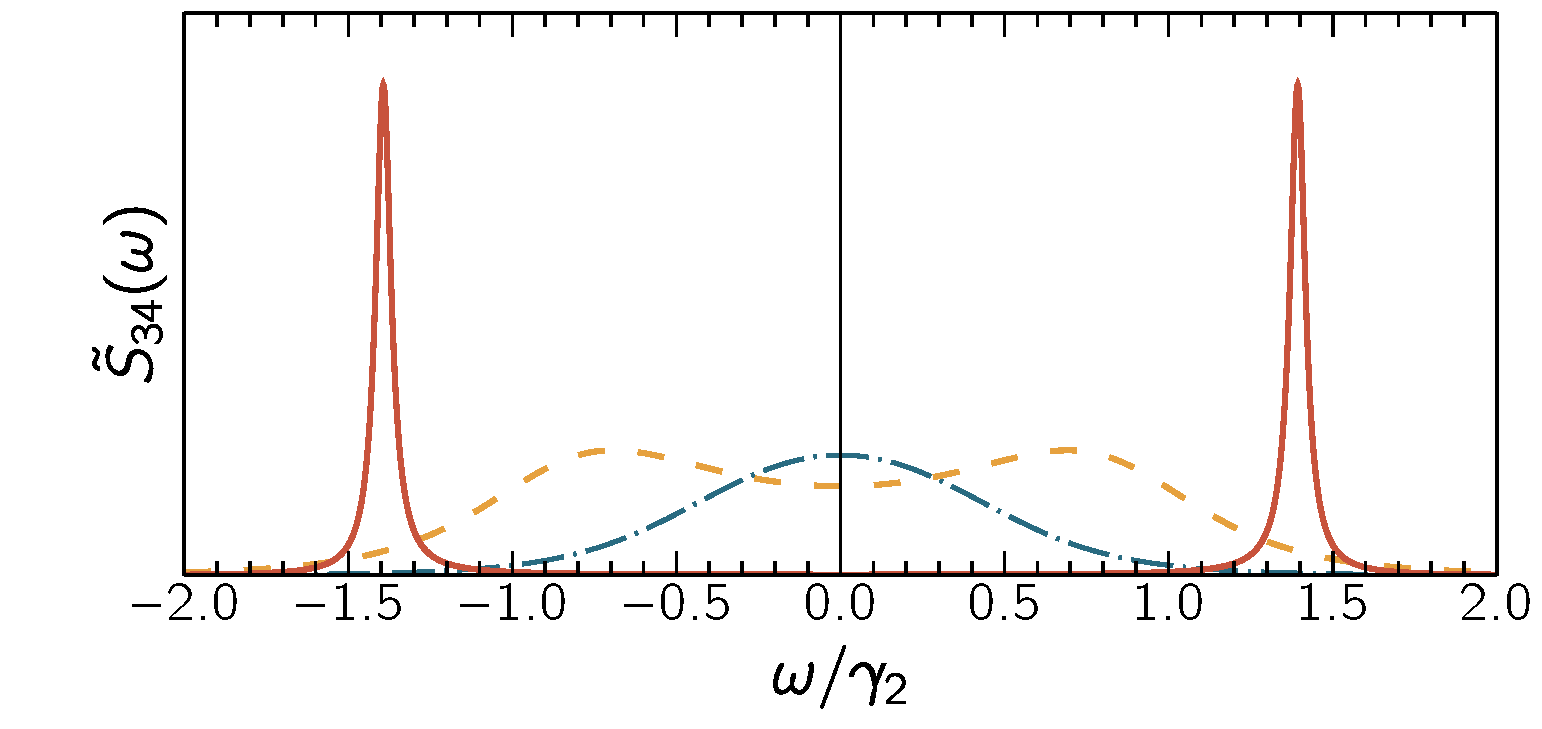
\includegraphics[width=0.64\textwidth]
	  {./figures/fig_3.pdf}}
	\subfigure{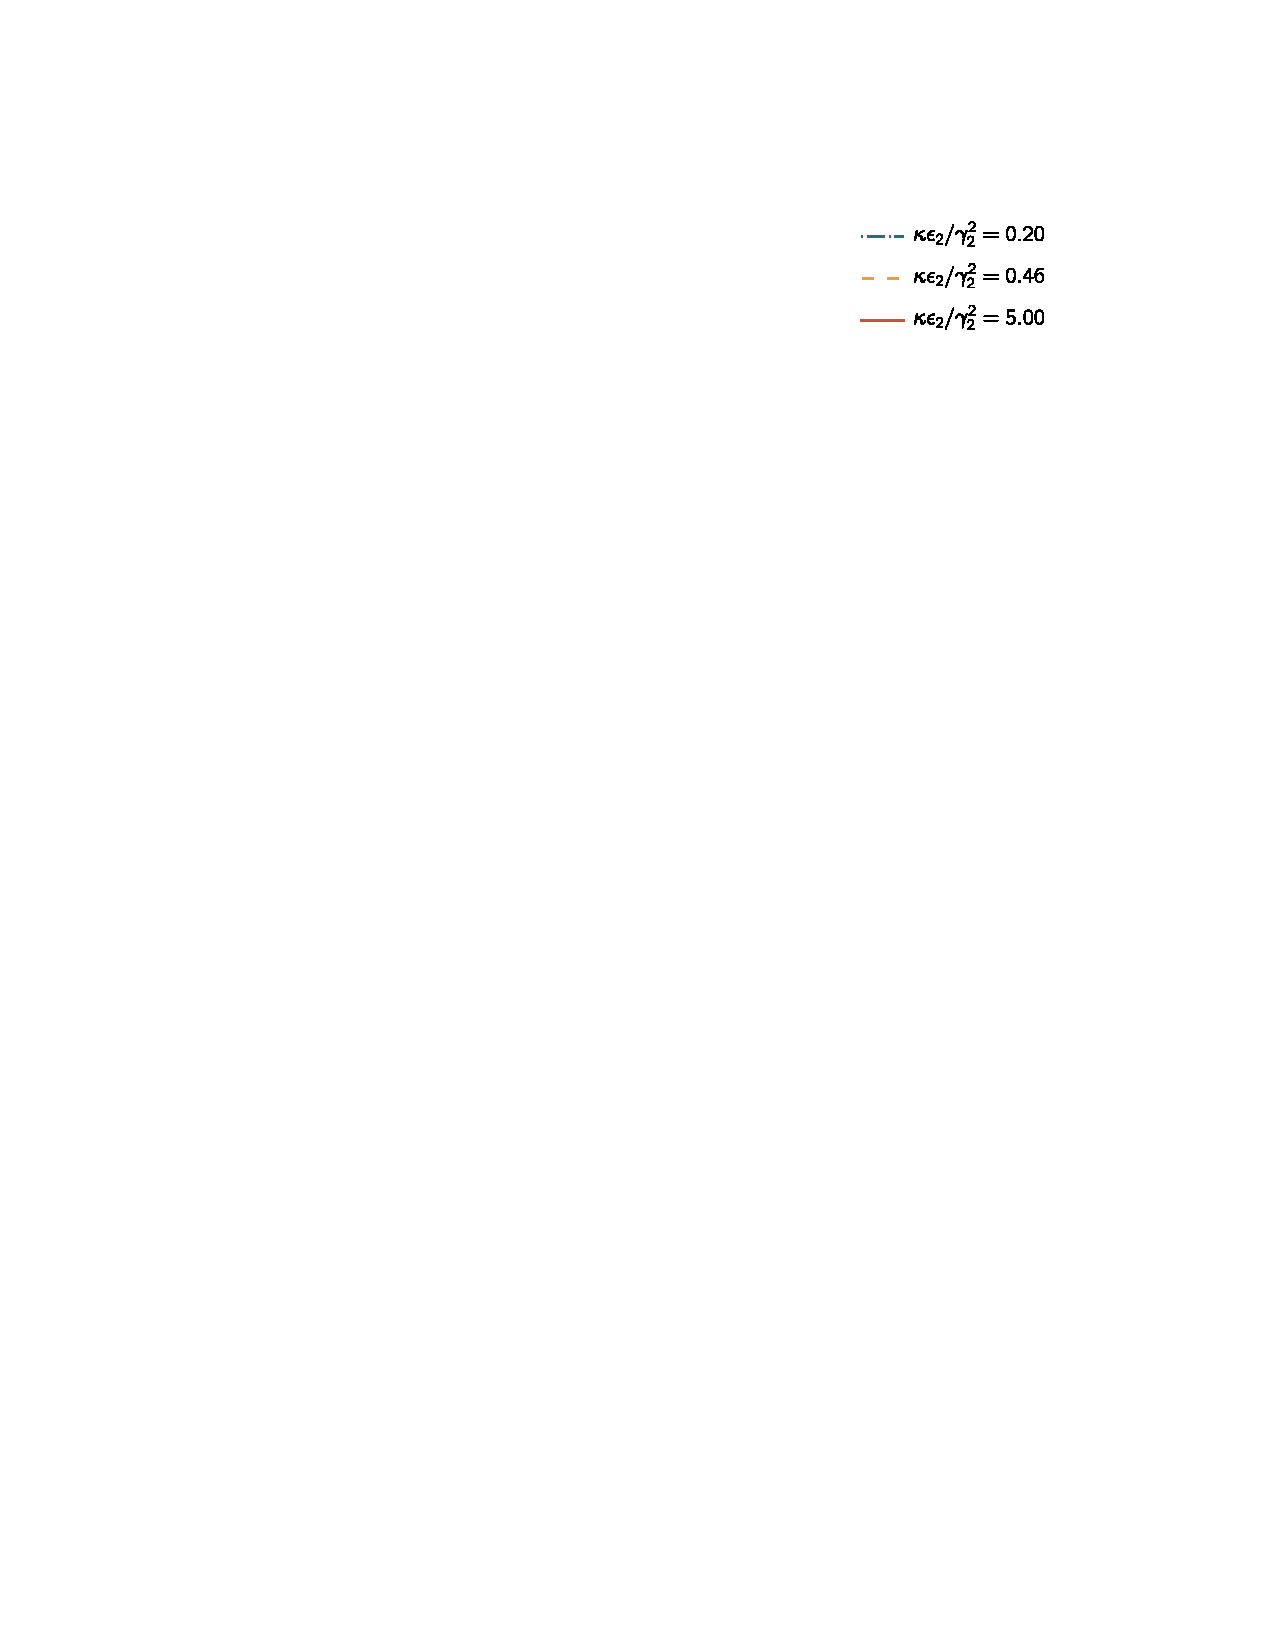
\includegraphics[width=0.18\textwidth]
	  {./figures/fig_3_legend.pdf}}
	\caption{Linearized spectrum $\tilde{S}_{34}(\tilde{\omega})$ for sub harmonic generation. Here, we assumed that $\gamma_1/\gamma_2 = 0.5$. Vertical scale ratios: 1:15:5000.}
	\label{fig_3}
\end{figure}

\section*{Discussion}

A comprehensive quantum statistical analysis has been conducted in this study to examine the phenomenon of coherently driven sub/second harmonic generation within an optical cavity. This research described the intricate dynamics of quantum fluctuations, particularly focusing on their behavior in proximity to the instability states as predicted by classical theory.

One significant observation is the spectrum of the subharmonic light, which undergoes a critical narrowing effect as it approaches the threshold for the second-order phase transition. In cavity nonlinear optics, second-order phase transitions may arise in systems that show spontaneous symmetry breaking, wherein the system transfer from one state to another with changes in a parameter. In this investigation, we manipulated the intensity of the driving field as this parameter. Understanding second-order phase transitions in cavity non-linear optics can provide insights into the complex behavior of light-matter interactions in confined geometries and can have implications for various applications, including the development of novel optical devices and technologies.
Furthermore, as the driving field intensity increases, the subharmonic spectrum separates into two distinct peaks, signifying a complex interplay of non-linear effects within the resonator. This phenomenon manifests as oscillations in the correlation functions when the eigenvalues of the linearized equations of motion acquire non-zero imaginary parts.

Moreover, the investigation showed a fascinating behavior in the spectrum of the second harmonic generation. Below the threshold for hard mode oscillations, the second harmonic spectrum similarly splits into two peaks, suggesting the emergence of distinct resonance modes within the system. In addition, the width of these peaks diminishes as the threshold is approached, indicating a progressive stabilization of the system towards a more coherent state. Understanding these dynamics could pave the way for novel applications in fields ranging from biomedical imaging to quantum computing.

This comprehensive theoretical analysis provided valuable insights into the complex dynamics of coherently driven sub/second harmonic generation within optical resonators. It illuminated the fundamental physics behind the emergence of intricate spectral characteristics and phase transitions in such systems.


\bibliography{manuscript}
\end{document}
